\chapter{REVISÃO BIBLIOGRÁFICA}
\label{cap1Revisao}

Na América Latina, historicamente marcada pela exploração colonial, o extrativismo mineral teve início para atender aos interesses dos países colonizadores. No final da década de 1990, com a expansão da globalização e o crescimento do consumo de metais, a indústria mineral passou a se expandir em ritmo acelerado, tanto em volume extraído quanto na abertura de novas minas \cite{fernandes2016mineracao}.

Em 2023, o Brasil ocupava a nona posição no ranking mundial de produtores de minerais metálicos e carvão \cite{wpr2024mineral}. O setor possuía importância estratégica para a economia nacional, gerando empregos e respondendo por parcela expressiva das exportações \cite{anm2023informe3}.

Conforme \citeauthor{carvalho2012dependencia} (\citeyear{carvalho2012dependencia}), a mineração produzia bens primários que supriam atividades econômicas desde a agricultura até a indústria de tecnologia de ponta, sendo um fator fundamental em economias baseadas na extração de recursos minerais.

% =============================================================
\section{Atividade de Mineração}
\label{sec:atividade_mineracao}
% =============================================================

A mineração no Brasil remonta ao período colonial, com a extração de ouro no século XVIII impulsionando a ocupação do território. 

Foi a partir do século XX, porém, que a relação entre o Estado e o setor se institucionalizou: o Código de Mineração de 1934 (Decreto Federal n.º 24.642) consolidou a legislação existente, conferiu ao governo o papel de fiscalizar os planos de trabalho e definiu formalmente os conceitos de ``jazida'' e ``mina'', instituindo a necessidade de autorização prévia para pesquisa mineral e concessão de lavra pelo DNPM \cite{brasil1934b, domingues2022}.

Sob o governo Vargas, a partir de 1930, o setor mineral foi integrado a um projeto nacionalista de desenvolvimento, com a criação da CVRD em 1942 e da Petrobras em 1954 como expressões dessa política \cite{villasboas1995, fonseca2012}. 

No período de Juscelino Kubitschek, a abertura ao capital estrangeiro marcou a transição para um ``capitalismo associado'', enquanto a Ditadura Militar (1964--1985) impulsionou grandes projetos exportadores, como a extração de minério de ferro em Carajás (1967) \cite{fernandes2016, domingues2022}. Os Códigos de Mineração de 1940 e 1967 representaram marcos adicionais de normatização \cite{brasil1967, domingues2022}.

A partir da redemocratização, em 1985, o Brasil consolidou-se como um dos principais produtores e exportadores globais de minerais. Entre 1985 e 2015, cerca de 85\% da produção mineral era exportada, com o minério de ferro constituindo 89\% dessa pauta \cite{fernandes2016}.

Na década de 1990, o conceito de desenvolvimento sustentável ganhou espaço no setor, impulsionado pelo projeto \textit{Mining, Minerals and Sustainable Development} (MMSD), coordenado pelo Centro de Tecnologia Mineral (CETEM), que estabeleceu novas perspectivas para a análise integrada da atividade extrativa \cite{barreto2001}.

Atualmente, o minério de ferro representa aproximadamente 60\% das exportações do setor mineral brasileiro, que constitui, junto ao agronegócio, um dos pilares estratégicos da balança comercial \cite{anm2023boletim}. 

Segundo o Instituto Brasileiro de Mineração \citeonline{ibram2024}, em 2024 o setor registrou faturamento de R\$~270,8 bilhões (alta de 9,1\% em relação a 2023), exportações minerais de US\$~43,43 bilhões e saldo comercial de US\$~34,9 bilhões, equivalente a 47\% do saldo total da balança comercial brasileira. O setor mantinha mais de 221 mil empregos diretos, com geração de 8.703 novas vagas entre janeiro e novembro de 2024. Os principais Estados produtores eram Minas Gerais (40\% do faturamento) e Pará (36,1\%) \cite{ibram2024}.

% -------------------------------------------------------------
\subsection{O papel da atividade mineradora na economia}
\label{subsec:papel_mineracao_economia}
% -------------------------------------------------------------

\subsubsection{Percentual do PIB devido à mineração}
\label{subsubsec:percentual_pib}

A mineração e a siderurgia respondiam conjuntamente por aproximadamente 3,1\% do PIB nacional, com a mineração contribuindo isoladamente com cerca de 1,2\% \cite{apc2024}. Entre 2000 e 2019, essa participação oscilou entre 2,5\% e 4\%, refletindo tanto os ciclos econômicos internos quanto as flutuações nas cotações internacionais de \textit{commodities} \cite{leao2023, ipea2023, apc2024}.

A metodologia desenvolvida pelo Instituto de Pesquisa Econômica Aplicada (IPEA) e pelo Ministério de Minas e Energia (MME) em 2023 avançou sobre as abordagens tradicionais ao utilizar a Matriz Insumo-Produto para calcular o ``arrasto produtivo'' --- a parcela do PIB gerada em outros setores estimulada pela economia mineral. Os resultados mostraram que a cadeia produtiva mineral representou entre R\$~150 bilhões e R\$~340 bilhões entre 2000 e 2019 (valores constantes de 2021), com destaque para o minério de ferro, cujo multiplicador econômico superava 1 ao longo de todo o período \cite{leao2023}.

\subsubsection{Mineração em números}
\label{subsubsec:mineracao_numeros}
 
Segundo os dados do IBRAM (\citeyear{ibram2024}) apud \citeonline{fonseca2024resultados}, em 2023 o faturamento da mineração brasileira manteve-se estável em R\$~248,2 bilhões (redução de 0,7\% em relação a 2022), com Minas Gerais respondendo por 41,7\% do total. As exportações minerais alcançaram US\$~43 bilhões, gerando saldo comercial de US\$~31,95 bilhões --- 32\% do saldo total da balança comercial de 2023. O minério de ferro correspondeu a 71\% dos minérios exportados, com volume de 378,5 milhões de toneladas, Figuras \ref{fig:image1_mineracao_numeros_1} e \ref{fig:image2_mineracao_numeros_2}. 

\begin{figure}[H]
    \centering
    \fbox{\includegraphics[width=0.97\textwidth]{figures/image1_mineracao_numeros_1.png}}
    \caption{Mineração em Números (2024) -- Saldo comercial, impostos e faturamento}
    \label{fig:image1_mineracao_numeros_1}
    \fonte{Mineração em Números (IBRAM, 2024)}
\end{figure}

\begin{figure}[H]
    \centering
    \fbox{\includegraphics[width=0.97\textwidth]{figures/image2_mineracao_numeros_2.png}}
    \caption{Mineração em Números (2024) -- Exportação e Importação}
    \label{fig:image2_mineracao_numeros_2}
    \fonte{Mineração em Números (IBRAM, 2024)}
\end{figure}

Os investimentos projetados para 2024--2028 chegam a US\$~64,5 bilhões, sendo 16,6\% destinados a iniciativas socioambientais. A Figura~\ref{fig:image3_mineracao_numeros_3} detalha a participação das principais substâncias produzidas no faturamento do setor.

\begin{figure}[H]
    \centering
    \fbox{\includegraphics[width=0.97\textwidth]{figures/image3_mineracao_numeros_3.png}}
    \caption{Mineração em Números (2024) -- Principais substâncias produzidas -- Participação no faturamento do setor}
    \label{fig:image3_mineracao_numeros_3}
    \fonte{Mineração em Números (IBRAM, 2024)}
\end{figure}

\subsubsection{Geração de empregos}
\label{subsubsec:geracao_empregos}

A análise do mercado de trabalho no setor mineral abrange a Indústria Extrativa Mineral (IEM) e a Indústria de Transformação Mineral (ITM), conforme metodologia da Agência Nacional de Mineração (ANM). Desde 2020, o monitoramento do emprego formal passou a ser feito pelo Novo CAGED (eSocial) \cite{anm2023informe3, anm2023informe4}.

\paragraph*{Emprego Formal na Indústria Extrativa Mineral (IEM)}

No 4.º trimestre de 2023, a IEM registrou estoque de 208.176 trabalhadores (Figura~\ref{fig:image5_saldo_estoque_4tri2023}), com saldo ligeiramente negativo de $-$119 vagas no período. No 3.º trimestre, o saldo havia sido positivo em 1.869 vagas (Figura~\ref{fig:saldo_estoque_3tri2023}) \cite{anm2023informe3, anm2023informe4}.


\begin{figure}[H]
    \centering
    \fbox{\includegraphics[width=0.97\textwidth]{figures/image5_saldo_estoque_4tri2023.png}}
    \caption{Saldo ajustado e estoque trimestral de mão de obra da IEM (exceto petróleo e gás) -- 04TRI2023}
    \label{fig:image5_saldo_estoque_4tri2023}
    \fonte{\citeauthor{anm2023informe4} (\citeyear{anm2023informe4})}
\end{figure}

\begin{figure}[H]
    \centering
    \fbox{\includegraphics[width=0.97\textwidth]{figures/image4_saldo_estoque_3tri2023.png}}
    \caption{Saldo ajustado e estoque trimestral de mão de obra da IEM (exceto petróleo e gás) -- 03TRI2023}
    \label{fig:saldo_estoque_3tri2023}
    \fonte{\citeauthor{anm2023informe3} (\citeyear{anm2023informe3})}
\end{figure}

A dinâmica do emprego na IEM era heterogênea entre seus subgrupos. No 3.º trimestre de 2023, a Extração de Minério de Ferro apresentou o maior saldo positivo (1.171 vagas), enquanto a Extração de Minerais Metálicos Não-Ferrosos registrou $-$653 vagas, impactada pela suspensão de operações da AngloGold Ashanti em Santa Bárbara (MG) e pela falência da Buritirama Mineração em Marabá (PA), conforme apresentado na Figura~\ref{fig:saldo_mao_obra_3tri2023}.

\begin{figure}[H]
    \centering
    \fbox{\includegraphics[width=0.97\textwidth]{figures/image6_saldo_mao_obra_3tri2023.png}}
    \caption{Saldo de mão de obra da IEM (exceto petróleo e gás), por grupo CNAE 2.0 -- 03TRI2023}
    \label{fig:saldo_mao_obra_3tri2023}
    \fonte{\citeauthor{anm2023informe3} (\citeyear{anm2023informe3})}
\end{figure}

Já na variação interanual do 4.º trimestre (2023 vs. 2022), destacou-se o crescimento de 12,7\% na Extração de Minério de Ferro e a queda de 38,6\% nas Atividades de Apoio (Figura~\ref{fig:variacao_emprego_4tri2023}) \cite{anm2023informe3, anm2023informe4}.

\begin{figure}[H]
    \centering
    \fbox{\includegraphics[width=0.97\textwidth]{figures/image7_variacao_emprego_4tri2023.png}}
    \caption{Variação interanual do emprego formal na IEM (exceto petróleo e gás), por grupo CNAE 2.0 -- 04TRI2023}
    \label{fig:variacao_emprego_4tri2023}
    \fonte{\citeauthor{anm2023informe4} (\citeyear{anm2023informe4})}
\end{figure}
 
A força de trabalho da IEM concentrava-se em Minas Gerais (35\%), Pará (13\%), Bahia (7\%) e São Paulo (7\%) (Figura~\ref{fig:estoque_mao_obra}) \cite{anm2023informe3}.
 
\begin{figure}[H]
    \centering
    \fbox{\includegraphics[width=0.97\textwidth]{figures/image8_estoque_mao_obra.png}}
    \caption{Estoque de mão de obra da IEM (exceto petróleo e gás) por estado}
    \label{fig:estoque_mao_obra}
    \fonte{\citeauthor{anm2023informe3} (\citeyear{anm2023informe3})}
\end{figure}

A mediana salarial de admissão na IEM foi de R\$~1.988,67 no 4.º trimestre de 2023, com valores superiores em subgrupos como Extração de Carvão Mineral (R\$~3.370,31) e Extração de Minério de Ferro (R\$~2.300,43) (Figura~\ref{fig:salarios_admissao}) \cite{anm2023informe4}.

\begin{figure}[H]
    \centering
    \fbox{\includegraphics[width=0.97\textwidth]{figures/image11_salarios_admissao.png}}
    \caption{Salários de admissão na extração mineral na IEM -- 04TRI2023}
    \label{fig:salarios_admissao}
    \fonte{\citeauthor{anm2023informe4} (\citeyear{anm2023informe4})}
\end{figure}

\FloatBarrier
\paragraph*{Indústria de Transformação Mineral (ITM)}

A ITM concentrava a maior parte da mão de obra formal do setor, registrando 718.631 postos no 4.º trimestre de 2023 (Figuras~\ref{fig:evolucao_saldo_itm} e~\ref{fig:evolucao_saldo_itm_3tri}). Os principais setores empregadores eram a fabricação de produtos cerâmicos, artefatos de concreto e a siderurgia. O estoque da ITM apresentou variação trimestral discreta ($-$0,3\% no 4.º trimestre de 2023), refletindo maior estabilidade em relação às flutuações da IEM \cite{anm2023informe3, anm2023informe4}.

\begin{figure}[H]
    \centering
    \fbox{\includegraphics[width=0.97\textwidth]{figures/image10_evolucao_saldo_itm.png}}
    \caption{Evolução do saldo e do estoque de trabalhadores da ITM -- 04TRI2022 a 04TRI2024}
    \label{fig:evolucao_saldo_itm}
    \fonte{\citeauthor{anm2023informe4} (\citeyear{anm2023informe4})}
\end{figure}

\begin{figure}[H]
    \centering
    \fbox{\includegraphics[width=0.97\textwidth]{figures/image10_evolucao_saldo_itm_3tri.png}}
    \caption{Evolução do saldo e do estoque de trabalhadores da ITM -- 03TRI2022 a 03TRI2024}
    \label{fig:evolucao_saldo_itm_3tri}
    \fonte{\citeauthor{anm2023informe3} (\citeyear{anm2023informe3})}
\end{figure}

A Indústria Extrativa Mineral contribui ainda de forma expressiva para as finanças públicas via CFEM (\textit{royalty} mineral), com arrecadação de R\$~1,80 bilhão no 4.º trimestre de 2023, concentrada em Minas Gerais e Pará (87,4\% do total) \cite{anm2023informe4}.

\FloatBarrier 
% -------------------------------------------------------------
\subsection{Geração de resíduos}
\label{subsec:geracao_residuos}
% -------------------------------------------------------------

A atividade minerária compreende, segundo o Decreto n.º 9.406/2018, as fases de pesquisa geológica, lavra, beneficiamento, transporte, comercialização, gestão de resíduos e fechamento da mina \cite{brasil2018}. As principais etapas do ciclo, ilustradas na Figura~\ref{fig:etapas_mineracao}, são a Prospecção, a Pesquisa Mineral, a Lavra e o Descomissionamento \cite{carvalho2018, freire2020}.

\begin{figure}[H]
    \centering
    \includegraphics[width=0.9\textwidth]{figures/image14_etapas_mineracao.png}
    \caption{Etapas da mineração.}
    \label{fig:etapas_mineracao}
    \fonte{\citeauthor{carvalho2018} (\citeyear{carvalho2018})}
\end{figure}

A Prospecção é a fase inicial, focada na busca por concentrações minerais de interesse econômico por meio de estudos geológicos preliminares. A Pesquisa Mineral aprofunda essa investigação, caracterizando o depósito e avaliando sua viabilidade econômica, sendo regulada pelo Regime de Autorização \cite{freire2020, anm2022}.

A Lavra é a etapa central do ciclo produtivo, englobando a extração das substâncias minerais úteis e seu beneficiamento (Figura~\ref{fig:operacoes_lavra}). É também a fase de maior geração de efluentes sólidos, líquidos e gasosos, exigindo Estudo de Impacto Ambiental (EIA) e licença ambiental prévia \cite{carvalho2018, freire2020}. Os métodos de lavra dividem-se em dois grandes grupos: lavra a céu aberto (superficial) e lavra subterrânea (Figura~\ref{fig:metodos_lavra}), sendo a céu aberto predominante no Brasil \cite{jr2019, freire2020, carvalho2018}.

\begin{figure}[H]
    \centering
    \includegraphics[width=0.9\textwidth]{figures/image16_operacoes_lavra.png}
    \caption{Operações de lavra.}
    \label{fig:operacoes_lavra}
    \fonte{\citeauthor{carvalho2018} (\citeyear{carvalho2018}), p. 344 apud \citeauthor{freire2020} (\citeyear{freire2020})}
\end{figure}

\begin{figure}[H]
    \centering
    \includegraphics[width=0.9\textwidth]{figures/image15_metodos_lavra.png}
    \caption{Métodos de Lavra.}
    \label{fig:metodos_lavra}
    \fonte{\citeauthor{jr2019} (\citeyear{jr2019}) apud \citeauthor{freire2020} (\citeyear{freire2020})}
\end{figure}

\FloatBarrier
\subsubsection{Resíduos sólidos de extração -- Estéril}

O estéril é o material retirado para dar acesso ao minério, sem valor econômico direto. Normalmente depositado em pilhas externas à mina, representa volumes expressivos da atividade de lavra a céu aberto e exige gestão ambiental adequada para evitar contaminação de solo e corpos d'água \cite{carvalho2018, freire2020}.

\subsubsection{Resíduos sólidos de beneficiamento -- Rejeito}

O rejeito é o resíduo resultante do processo de beneficiamento do minério, após a separação das frações de interesse econômico. Sua composição física e química varia conforme o tipo de minério processado, e seu armazenamento em barragens de contenção representa um dos principais desafios de segurança da mineração \cite{carvalho2018, freire2020}.

\subsubsection{Geração de resíduos sólidos}

A geração de resíduos sólidos na mineração é expressiva, especialmente no minério de ferro, que responde pela maior parte do volume de estéril e rejeito produzidos no Brasil. A gestão adequada desses materiais é regulada pela Política Nacional de Resíduos Sólidos e pelas normas específicas do setor mineral \cite{carvalho2018}.

\subsubsection{Gestão de resíduos e métodos de disposição de rejeitos}

Os métodos de disposição de rejeitos incluem o empilhamento a seco (\textit{dry stacking}), a pasta espessada e o armazenamento em barragens convencionais. O empilhamento a seco, embora mais custoso, tem sido progressivamente adotado por minimizar riscos de ruptura. As barragens convencionais, amplamente utilizadas pela sua relação custo-benefício, exigem monitoramento contínuo e instrumentação geotécnica \cite{carvalho2018, freire2020}.

% -------------------------------------------------------------
\subsection{Tipos de barragens de rejeitos}
\label{subsec:tipos_barragens}
% -------------------------------------------------------------

As barragens de contenção de rejeitos são estruturas geotécnicas destinadas ao armazenamento dos resíduos do beneficiamento mineral. Diferentemente das barragens de água convencional, são construídas de forma progressiva, com alteamentos sucessivos ao longo da vida útil da mina.

Os três principais métodos construtivos são o alteamento a montante, a jusante e pela linha de centro, diferindo fundamentalmente na direção em que o maciço da barragem se expande ao longo dos alteamentos (Figuras~\ref{fig:metodo_montante},~\ref{fig:metodo_jusante} e~\ref{fig:metodo_linha_de_centro}).

\subsubsection{Método de Alteamento a Montante}

No método a montante (Figura~\ref{fig:metodo_montante}), os diques de alteamento são construídos sobre a praia de rejeitos previamente depositados, avançando em direção ao reservatório. É o método de menor custo e maior velocidade de alteamento, mas apresenta vulnerabilidades estruturais significativas: a fundação sobre rejeitos não consolidados reduz a resistência ao cisalhamento e eleva o risco de liquefação, especialmente quando saturados. A implementação de sistemas de drenagem interna eficientes é também dificultada por esse método \cite{araujo2006, ibram2016}.

\begin{figure}[H]
    \centering
    \fbox{\includegraphics[width=0.9\textwidth]{figures/image18_metodo_montante.png}}
    \caption{Seção típica de uma barragem alteada a montante.}
    \label{fig:metodo_montante}
    \fonte{\citeauthor{albuquerque2004} (\citeyear{albuquerque2004})}
\end{figure}

\subsubsection{Método de Alteamento a Jusante}

No método a jusante (Figura~\ref{fig:metodo_jusante}), os alteamentos são construídos integralmente para fora do reservatório, sobre o dique de partida ou materiais de empréstimo. Isso permite controle mais rigoroso da compactação e instalação de sistemas de drenagem interna ao longo de toda a construção, resultando em maior estabilidade e resistência sísmica. Em contrapartida, exige volume maior de material e tem custo mais elevado \cite{araujo2006, ibram2016, ctsufsj2017}.

\begin{figure}[H]
    \centering
    \fbox{\includegraphics[width=0.9\textwidth]{figures/image19_jusante.png}}
    \caption{Seção típica de uma barragem alteada para jusante.}
    \label{fig:metodo_jusante}
    \fonte{\citeauthor{albuquerque2004} (\citeyear{albuquerque2004})}
\end{figure}

\subsubsection{Método de Alteamento pela Linha de Centro}

O método pela linha de centro (Figura~\ref{fig:metodo_linha_de_centro}) mantém o eixo da crista na mesma posição horizontal enquanto a barragem cresce em altura, com os alteamentos avançando levemente para jusante. Representa uma solução intermediária em custo e risco: supera o método a montante por não avançar continuamente sobre rejeito saturado, mas pode envolver fundação parcial sobre rejeitos parcialmente consolidados, o que o torna potencialmente menos seguro que o método a jusante \cite{soares2010, duarte2008, ctsufsj2017}.

\begin{figure}[H]
    \centering
    \fbox{\includegraphics[width=0.9\textwidth]{figures/image20_linha_de_centro.png}}
    \caption{Seção típica de uma barragem alteada pela linha de centro.}
    \label{fig:metodo_linha_de_centro}
    \fonte{\citeauthor{albuquerque2004} (\citeyear{albuquerque2004})}
\end{figure}

\FloatBarrier
\subsubsection{Características, vantagens e desvantagens dos três métodos}

As Tabelas~\ref{tab:caracteristicas_barragens} e~\ref{tab:vantagens_desvantagens} sintetizam as características, vantagens e desvantagens dos três métodos.

% Tabela 1
\begin{table}[h!]
    \centering
    \caption{Características dos principais métodos construtivos de barragens de rejeitos}
    \label{tab:caracteristicas_barragens}
    \begin{tabular}{|p{3.8cm}|p{3.3cm}|p{3.3cm}|p{3.3cm}|}
        \hline
        \textbf{Características} & \textbf{Montante} & \textbf{Jusante} & \textbf{Linha de Centro} \\
        \hline
        \textbf{Tipo de rejeito recomendado} &
        Baixa densidade; segregação; mais de 40\% de areia &
        Qualquer tipo &
        Lamas de baixa plasticidade \\
        \hline
        \textbf{Descarga de rejeitos} &
        Periférica &
        De acordo com o projeto &
        Periférica, conservando o eixo \\
        \hline
        \textbf{Armazenamento de água} &
        Não recomendável para grandes volumes &
        Bom &
        Aceitável; não recomendado para armazenamento permanente \\
        \hline
        \textbf{Resistência sísmica} &
        Baixa &
        Boa &
        Aceitável \\
        \hline
        \textbf{Alteamentos} &
        Ideal $<$10~m/ano; perigoso $>$15~m/ano &
        Sem restrição &
        Pouca restrição \\
        \hline
        \textbf{Custo relativo} &
        Baixo ($V_m$) &
        Alto (3$V_m$) &
        Moderado (2$V_m$) \\
        \hline
    \end{tabular}
    \footnotesize
    Fonte: Adaptado de \citeauthor{freire2020} (\citeyear{freire2020}) e \citeauthor{lozano2006} (\citeyear{lozano2006}).
\end{table}

% Tabela 2
\begin{table}[h!]
    \centering
    \caption{Vantagens e desvantagens dos três tipos de barragens de rejeitos}
    \label{tab:vantagens_desvantagens}
    % \begin{tabular}{|p{2.4cm}|p{3.75cm}|p{3.75cm}|p{3.75cm}|}
    \begin{tabular}{|p{3.8cm}|p{3.3cm}|p{3.3cm}|p{3.3cm}|}
        \hline
         & \textbf{Montante} & \textbf{Jusante} & \textbf{Linha de Centro} \\
        \hline
        \textbf{Método} &
        Mais antigo e amplamente empregado. Alteamentos periféricos sobre rejeitos via ciclonagem. &
        Dique impermeável + barragem de pé; dreno interno e impermeabilização a montante. &
        Variação do método a jusante. \\
        \hline
        \textbf{Vantagens} &
        Menor custo; maior velocidade de alteamento. &
        Maior segurança; compactação integral; permite mistura com estéreis. &
        Volume de \textit{underflow} inferior ao método a jusante. \\
        \hline
        \textbf{Desvantagens} &
        Linha freática próxima ao talude; susceptibilidade a liquefação e \textit{piping}. &
        Grande quantidade de \textit{underflow}; proteção superficial apenas no final. &
        Exige sistemas de drenagem eficientes e contenção a jusante. \\
        \hline
    \end{tabular}
    \footnotesize
    Fonte: Adaptado de \citeauthor{lozano2006} (\citeyear{lozano2006}).
\end{table}

\FloatBarrier
\subsubsection{Método de Alteamento ``Etapa Única''}

Além dos três métodos progressivos, existe o método ``Etapa Única'' (\textit{Single Stage}), no qual a barragem é construída até a altura final em uma única fase, em solo compactado ou enrocamento. É utilizado em instalações de menor porte e não permite expansão futura da capacidade de armazenamento \cite{vale2024, teck2019}, conforme apresentado na Figura~\ref{fig:metodo_etapa_unica}.

\begin{figure}[H]
    \centering
    \fbox{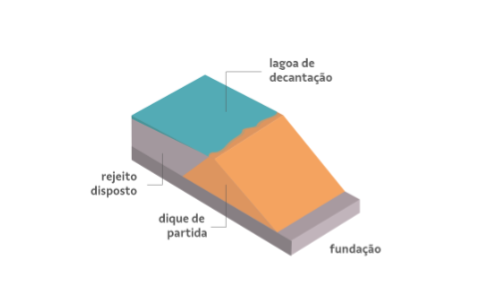
\includegraphics[width=\textwidth]{figures/image18_metodo_etapa_unica.png}}
    \caption{Seção típica de uma barragem alteada em ``Etapa Única''.}
    \label{fig:metodo_etapa_unica}
    \fonte{\citeauthor{vale2026glossario} (\citeyear{vale2026glossario})}
\end{figure}

% -------------------------------------------------------------
\FloatBarrier
\subsection{Panorama Brasil vs. Mundo}
% -------------------------------------------------------------

Grandes mineradoras como Vale S.A. e Teck Resources empregam diferentes métodos construtivos adaptados às condições geotécnicas de cada empreendimento \cite{vale2024, teck2019}. O método a montante, embora de menor custo, apresenta limitações estruturais que o tornaram proibido em países com alta atividade sísmica, como Chile e Peru \cite{thome2018}.

No Brasil, o Decreto Estadual n.º~46.993/2016 de Minas Gerais instituiu auditorias extraordinárias de segurança para barragens com alteamento a montante \cite{thome2018}. Após os desastres de Mariana (2015) e Brumadinho (2019), a Lei n.º~14.066/2020 proibiu formalmente a construção ou alteamento de barragens pelo método a montante e determinou a descaracterização das estruturas existentes, com prazo inicial até fevereiro de 2022. Minas Gerais estabeleceu prazo ainda mais exíguo pela Lei Estadual n.º~23.291/2019 (fevereiro de 2021), com prorrogações mediante termos de compromisso com o Ministério Público \cite{anm2023boletim, cbhsf2020, feam2024}.

Segundo consulta ao Sistema Integrado de Gestão de Barragens de Mineração (SIGBM) em maio de 2025, a construção em etapa única era o método mais utilizado (53,9\%), seguido pelo alteamento a jusante (23,8\%) e pela linha de centro (12,4\%), conforme apresentado na Figura~\ref{fig:distribuicao_barragens}. As estruturas com alteamento a montante correspondiam a apenas 5,6\% do total cadastrado \cite{anmsistema2020}.

\begin{figure}[H]
    \centering
    \fbox{\includegraphics[width=\textheight, height=\textwidth, keepaspectratio, angle=-90]{figures/image21_distribuicao_barragens_por_metodo_atual.png}}
    \caption{Distribuição das barragens por método construtivo}
    \label{fig:distribuicao_barragens}
    \fonte{\citeauthor{anmsistema2020} (\citeyear{anmsistema2020})}
\end{figure}

% =============================================================
\section{Classificação de risco das barragens de rejeitos}
\label{sec:classificacao_risco}
% =============================================================

\subsection{Estrutura Regulatória Contemporânea}
\label{sec:legislacao}

A regulamentação da mineração no Brasil acompanhou a evolução do ordenamento jurídico nacional. A Constituição de 1891 vinculava a propriedade do subsolo à do solo; o Código de Mineração de 1934 separou formalmente esses domínios, estabelecendo o controle estatal sobre os recursos minerais e criando o Departamento Nacional de Produção Mineral (DNPM) \cite{mme2025linha}. O período getulista consolidou o controle estatal, com a Constituição de 1937 restringindo a participação estrangeira na mineração \cite{mme2025linha}.

A preocupação ambiental ganhou força na legislação a partir da Conferência de Estocolmo (1972) e, no Brasil, com a Lei Federal n.º~6.938/1981, que instituiu a Política Nacional do Meio Ambiente (PNMA) e tornou obrigatória a recuperação ambiental das áreas mineradas. A Resolução do Conselho Nacional do Meio Ambiente (CONAMA) n.º~001/1986 estabeleceu a obrigatoriedade do Estudo de Impacto Ambiental e respectivo Relatório de Impacto Ambiental (EIA/RIMA) para atividades de extração mineral \cite{barros2017legislacao, conama1986resolucao001}.

A Constituição Federal de 1988 formalizou o direito ao meio ambiente equilibrado e a responsabilidade objetiva por danos ambientais (art. 225), reafirmando a obrigação de recuperação das áreas degradadas pela mineração \cite{brasil1988constituicao}.

A Lei n.º~9.605/1998 (Lei de Crimes Ambientais) tipificou condutas como a extração sem licença e o não cumprimento de obrigações de recuperação ambiental \cite{brasil1998lei9605}. A Lei n.º~12.334/2010 estabeleceu a Política Nacional de Segurança de Barragens (PNSB), criando o Sistema Nacional de Informações sobre Segurança de Barragens (SNISB) e critérios de classificação por risco e dano potencial \cite{brasil2010pnsb}.
 
É importante destacar que a PNSB, desde sua criação, aplicava-se de forma unificada a três categorias distintas de estruturas: barragens de acumulação de água para quaisquer usos, barragens de disposição de rejeitos de mineração e barragens de acumulação de resíduos industriais (art. 1º, parágrafo único, da Lei n.º~12.334/2010). Embora os princípios gerais de classificação por categoria de risco e dano potencial associado fossem comuns às três categorias, a fiscalização e o detalhamento técnico da metodologia de cálculo eram atribuídos a órgãos distintos conforme a finalidade da estrutura — cabendo à Agência Nacional de Águas (ANA) as barragens de acumulação hídrica e à Agência Nacional de Mineração (ANM) as barragens de rejeitos de mineração (art. 5º da Lei n.º~12.334/2010) \cite{brasil2010pnsb}.

A norma NBR~13028:2017 complementou esse marco com diretrizes técnicas específicas para projetos, análise de estabilidade e planos de emergência \cite{brasil2010pnsb, abnt2017}.

Após os desastres de 2015 e 2019, a Lei n.º~14.066/2020 reformulou profundamente a PNSB, proibindo o método a montante, exigindo a descaracterização das estruturas existentes e ampliando os requisitos de monitoramento. A ANM implementou o Sistema Integrado de Gestão de Segurança de Barragens de Mineração (SIGBM) como ferramenta central de gestão e classificação das barragens, incorporando painéis de \textit{Business Intelligence} e exigindo documentação periódica como a Declaração de Condição de Estabilidade (DCE) \cite{brasil2020lei14066, anmsistema2020}.

\subsection{Classificação das barragens de rejeitos}

A Lei n.º~12.334/2010 definiu, em seu art. 2º, os dois conceitos centrais usados na classificação de qualquer barragem sujeita à PNSB (Figura~\ref{fig:classificacao_barragens}). A categoria de risco foi definida como a classificação da estrutura em função dos aspectos que pudessem influenciar a possibilidade de ocorrência de acidente, considerando as características técnicas, os métodos construtivos, o estado de conservação e a idade do empreendimento, além do atendimento ao Plano de Segurança da Barragem (art. 2º, VIII, e art. 7º, §1º, com a redação dada pela Lei n.º~14.066/2020). O dano potencial associado, por sua vez, foi definido como o dano que poderia ocorrer devido a rompimento, vazamento, infiltração no solo ou mau funcionamento de uma barragem, independentemente de sua probabilidade de ocorrência, graduado de acordo com as perdas de vidas humanas e os impactos sociais, econômicos e ambientais (art. 2º, VII) \cite{brasil2010pnsb, brasil2020lei14066}.

\begin{figure}[H]
    \centering
    \fbox{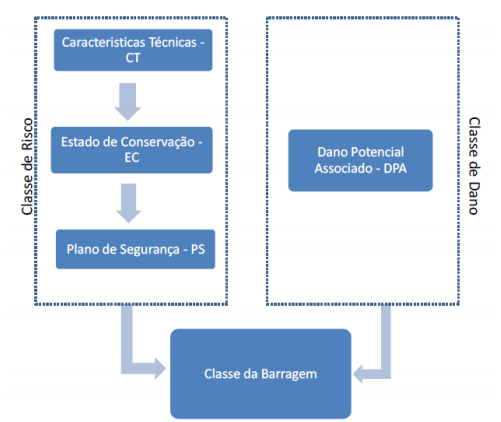
\includegraphics[width=0.97\textwidth]{figures/image26_classificacao_barragens.png}}
    \caption{Fluxograma de aplicação da classificação estabelecida pela Resolução 143/CNRH}
    \label{fig:classificacao_barragens}
    \fonte{\cite{moecke2019} de acordo com Resolução n.º~143 CNRH}
\end{figure}

Para as barragens de rejeitos de mineração, a ANM regulamentou esses dois critérios por meio da Portaria DNPM n.º~70.389/2017, que estabeleceu um método quantitativo de pontuação para a Categoria de Risco (CRI) e para o Dano Potencial Associado (DPA), expresso pelas Equações~\ref{eq:classe_risco} e~\ref{eq:classe_dano} \cite{brasil2017portaria70389}:

A Categoria de Risco (CRI) resulta da soma de três dimensões independentes, cada uma composta por parâmetros pontuados de 0 (condição mais segura) a 10 (condição mais crítica), expresso pela Equação~\ref{eq:classe_risco}.

\begin{equation}
\text{CRI} = \sum CT + \sum EC + \sum PS
\label{eq:classe_risco}
\end{equation}

A dimensão \textbf{Características Técnicas (CT)} considera cinco parâmetros da estrutura: a altura do maciço (a), o comprimento da crista (b), a vazão de projeto adotada (c), o método construtivo empregado (d) e a confiabilidade da instrumentação de auscultação instalada (e), conforme Equação~\ref{eq:classe_ct}. O método construtivo é o parâmetro de maior peso relativo: enquanto a construção em etapa única recebe pontuação mínima, o alteamento a montante ou de método desconhecido recebe a pontuação máxima (10 pontos).

\begin{equation}
\text{CT} = \sum_{i=a}^{e} X_i
\label{eq:classe_ct}
\end{equation}

A dimensão \textbf{Estado de Conservação (EC)} avalia a condição física atual da barragem por meio de quatro critérios: a confiabilidade das estruturas extravasoras (f), a existência e o controle de percolação (g), a presença de deformações e recalques (h), e o grau de deterioração dos taludes e paramentos (i), conforme Equação~\ref{eq:classe_ec}. Qualquer anomalia classificada com pontuação máxima (10 pontos) em um desses quatro critérios implica a reclassificação automática da barragem para Categoria de Risco Alta, independentemente da pontuação total nas demais dimensões, e enseja a realização obrigatória de Inspeção de Segurança Especial.

\begin{equation}
\text{EC} = \sum_{y=f}^{i} X_y
\label{eq:classe_ec}
\end{equation}

A dimensão \textbf{Plano de Segurança (PS)} mensura a completude da documentação e da governança de segurança, considerando cinco aspectos: a existência de documentação de projeto (do projeto conceitual ao ``como construído'') (j), a estrutura organizacional e a qualificação técnica da equipe de segurança (k), a existência de manuais de procedimentos de inspeção e monitoramento (l), a existência de Plano de Ação Emergencial (PAE) quando exigido pelo órgão fiscalizador (m), e a regularidade na emissão de relatórios de inspeção e de análise de segurança da instrumentação (n), conforme Equação~\ref{eq:classe_ps}.

\begin{equation}
\text{PS} = \sum_{i=j}^{n} X_i
\label{eq:classe_ps}
\end{equation}

A soma das três dimensões define a faixa de classificação da CRI (Figura~\ref{fig:classificacao_cri}): Alta (pontuação total maior ou igual a 65, ou pontuação máxima em qualquer critério isolado de EC), Média (entre 38 e 64 pontos) e Baixa (até 37 pontos) \cite{brasil2017portaria70389}.

\begin{figure}[H]
    \centering
    \fbox{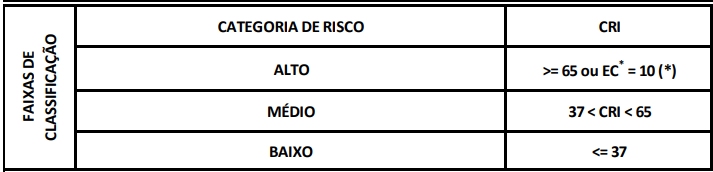
\includegraphics[width=0.97\textwidth]{figures/image27_classificacao_cri.png}}
    \caption{Faixa de classificação de risco}
    \label{fig:classificacao_cri}
    \fonte{\cite{brasil2017portaria70389}}
\end{figure}

O Dano Potencial Associado (DPA), por outro lado, independe das condições físicas da barragem e considera exclusivamente as consequências de uma eventual ruptura, a partir de quatro critérios: o volume total do reservatório (a), a existência de população a jusante (b), o impacto ambiental — relacionado à presença de áreas protegidas na área afetada (c) e à classe de periculosidade do rejeito armazenado (d), segundo a NBR~10.004 da ABNT — e o impacto socioeconômico das instalações existentes na área potencialmente atingida, expresso pela Equação~\ref{eq:classe_dano} \cite{brasil2017portaria70389}. 

\begin{equation}
\text{DPA} = \sum_{i=a}^{d} X_i
\label{eq:classe_dano}
\end{equation}

A soma desses quatro critérios define a faixa de DPA (Figura~\ref{fig:classificacao_dpa}): Alto (13 pontos ou mais), Médio (entre 8 e 12 pontos) e Baixo (até 7 pontos) \cite{brasil2017portaria70389}.

\begin{figure}[H]
    \centering
    \fbox{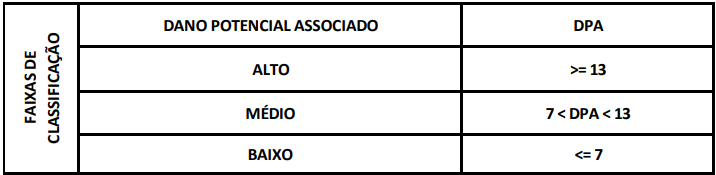
\includegraphics[width=0.97\textwidth]{figures/image27_classificacao_dpa.png}}
    \caption{Faixa de classificação de dano}
    \label{fig:classificacao_dpa}
    \fonte{\cite{brasil2017portaria70389}}
\end{figure}

A combinação entre a Categoria de Risco e o Dano Potencial Associado resulta, por fim, na classificação da barragem em cinco classes (A a E), apresentada na Figura~\ref{fig:classificacao_risco_dpa}, sendo a classe ``A'' reservada às barragens de maior risco e dano potencial combinados \cite{brasil2017portaria70389}.
 
\begin{figure}[H]
    \centering
    \fbox{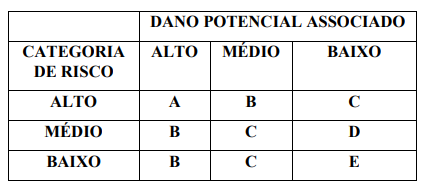
\includegraphics[width=0.8\textwidth]{figures/image27_classificacao_categoria_risco_dpa.png}}
    \caption{Classificação das barragens de mineração de acordo com a categoria de risco e o dano potencial associado}
    \label{fig:classificacao_risco_dpa}
    \fonte{\cite{brasil2017portaria70389}}
\end{figure}

\subsection{Panorama Atual de Classificação das Barragens de Mineração}

O Relatório Mensal da ANM de fevereiro de 2025 registrou 917 barragens de mineração cadastradas no SIGBM, das quais 467 (51\%) estavam inseridas na PNSB \cite{anm2025boletim}. A distribuição geográfica (Figura~\ref{fig:distribuicao_barragens_marco_2025}) reflete a vocação minerária histórica de cada estado: Minas Gerais concentrava o maior número, seguido por Mato Grosso, Pará, Bahia e São Paulo \cite{anm2025boletim}.

\begin{figure}[H]
    \centering
    \fbox{\includegraphics[width=\textwidth]{figures/image28_distribuicao_barragens_marco_2025.png}}
    \caption{Distribuição das barragens cadastradas no SIGBM em 05/03/2025.}
    \label{fig:distribuicao_barragens_marco_2025}
    \fonte{\cite{anm2025boletim}}
\end{figure}

As Figuras~\ref{fig:distribuicao_barragens_classificacao_cri} e~\ref{fig:distribuicao_barragens_classificacao_cri_estado} apresentam a distribuição por CRI no âmbito nacional e por estado, respectivamente. 

\begin{figure}[H]
    \centering
    \fbox{\includegraphics[width=0.9\textwidth]{figures/image29_distribuicao_barragens_classificacao_cri.png}}
    \caption{Distribuição de barragens cadastradas de acordo com sua classificação de CRI.}
    \label{fig:distribuicao_barragens_classificacao_cri}
    \fonte{\cite{anm2025boletim}}
\end{figure}

\begin{figure}[H]
    \centering
    \fbox{\includegraphics[width=\textwidth]{figures/image30_distribuicao_barragens_classificacao_cri_estado.png}}
    \caption{Distribuição das barragens inseridas na PNSB por estado, segundo a classificação de CRI.}
    \label{fig:distribuicao_barragens_classificacao_cri_estado}
    \fonte{\cite{anm2025boletim}}
\end{figure}

Minas Gerais destacava-se pelo maior número absoluto de barragens em CRI alto, reflexo de seus grandes complexos mineradores e do histórico recente de acidentes. Já o Pará apresentava maior proporção de estruturas em risco médio e baixo, em razão do predomínio de empreendimentos mais recentes \cite{anm2025boletim}.

Em fevereiro de 2025, a implementação da regra de classificação automática como CRI Alto por falta de envio da DCE (Resolução ANM n.º~95/2022, alterada pela Resolução n.º~175/2024) elevou o número de barragens nessa categoria. A evolução da CRI nos últimos 12 meses foi ilustrada na Figura~\ref{fig:evolucao_classificacao} \cite{anm2025boletim}.

\begin{figure}[H]
    \centering
    \fbox{\includegraphics[width=0.9\textwidth]{figures/image31_evolucao_classificacao_12_meses.png}}
    \caption{Evolução da classificação de CRI ao longo dos últimos 12 meses.}
    \label{fig:evolucao_classificacao}
    \fonte{\cite{anm2025boletim}}
\end{figure}

Em março de 2025, 104 barragens encontravam-se em situação de alerta ou emergência (Figura~\ref{fig:distribuicao_alerta}), das quais apenas duas em Nível 3 (Serra Azul/ArcelorMittal em Itatiaiuçu/MG e Forquilha III/Vale em Ouro Preto/MG) e seis em Nível 2 \cite{anm2025boletim}.

\begin{figure}[H]
    \centering
    \fbox{\includegraphics[width=\textwidth]{figures/image32_distribuicao_barragens_nivel_alerta.png}}
    \caption{Distribuição das barragens em nível de alerta ou emergência por estado em 05/03/2025.}
    \label{fig:distribuicao_alerta}
    \fonte{\cite{anm2025boletim}}
\end{figure}

\FloatBarrier 
\subsection{Risco: Severidade x Probabilidade}
\label{subsec:risco}

O risco é definido como o produto entre a probabilidade de ocorrência de um evento perigoso e a severidade de suas consequências \cite{sistemaeso2021avaliacao, sistemaeso2021matriz}. Na mineração, a quantificação do risco considera cenários estático, hidrológico, sísmico e de operação e manutenção, utilizando métodos como APR (\textit{Análise Preliminar de Risco}) e BTA (\textit{Bow-Tie Analysis}) para identificação e graduação dos cenários \cite{conceicao2018, vilaca2021}.

A severidade em eventos minerários manifesta-se em múltiplas dimensões: segurança dos trabalhadores, impactos ambientais, consequências sociais, aspectos legais e financeiros e reputação corporativa \cite{vilaca2021}. A metodologia RBPS exemplifica a complexidade dessas avaliações, com índices de falha variando entre 375,66 e 455,18 pontos para diferentes estruturas, e potencial de afetar até 12.900 pessoas em casos extremos \cite{conceicao2018}.

As normas ISO~31000 fornecem um \textit{framework} estruturado para gestão de riscos aplicável ao setor mineral, orientando a identificação, avaliação e tratamento dos riscos de forma sistemática \cite{cruz2024iso, ministeriotransportes2018}.

% =============================================================

\section{Mecanismos e casos de ruptura em barragens}
\label{sec:acidentes}
% =============================================================

Os mecanismos de ruptura em barragens geralmente atuam de forma combinada, amplificando seus efeitos individuais. Os três tipos fundamentais são a erosão interna, a liquefação e o galgamento \cite{arnez1999avaliacao}.

A \textbf{erosão interna} (\textit{piping}), apresentada na Figura~\ref{fig:erosao_piping}, ocorre pela remoção progressiva de partículas finas por gradientes hidráulicos elevados, criando canais preferenciais de fluxo que comprometem a integridade estrutural de dentro para fora \cite{arnez1999avaliacao}.

\begin{figure}[H]
    \centering
    \fbox{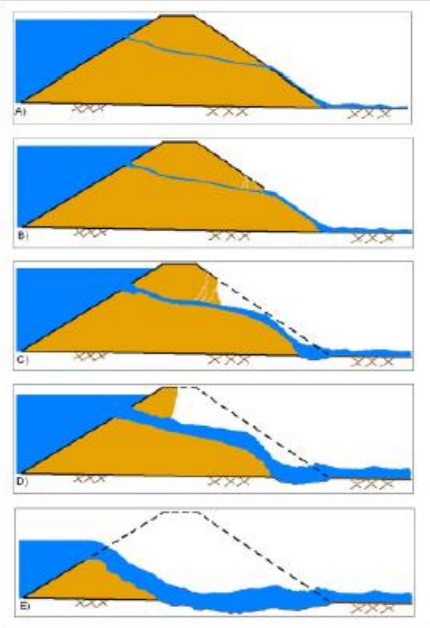
\includegraphics[width=0.4\textwidth]{figures/image_ruptura_erosao_piping.png}}
    \caption{Ruptura de barragem por erosão interna (\textit{piping}).}
    \label{fig:erosao_piping}
    \fonte{\cite{lara2016metodologia}}
\end{figure}

A \textbf{liquefação} é a perda súbita de resistência ao cisalhamento em solos saturados submetidos a carregamentos dinâmicos, como vibrações sísmicas, que transformam o material sólido em estado quase-líquido. Sua característica mais crítica é a rapidez e o grande volume afetado simultaneamente \cite{arnez1999avaliacao}, representada na Figura~\ref{fig:liquefacao}.

\begin{figure}[H]
    \centering
    \fbox{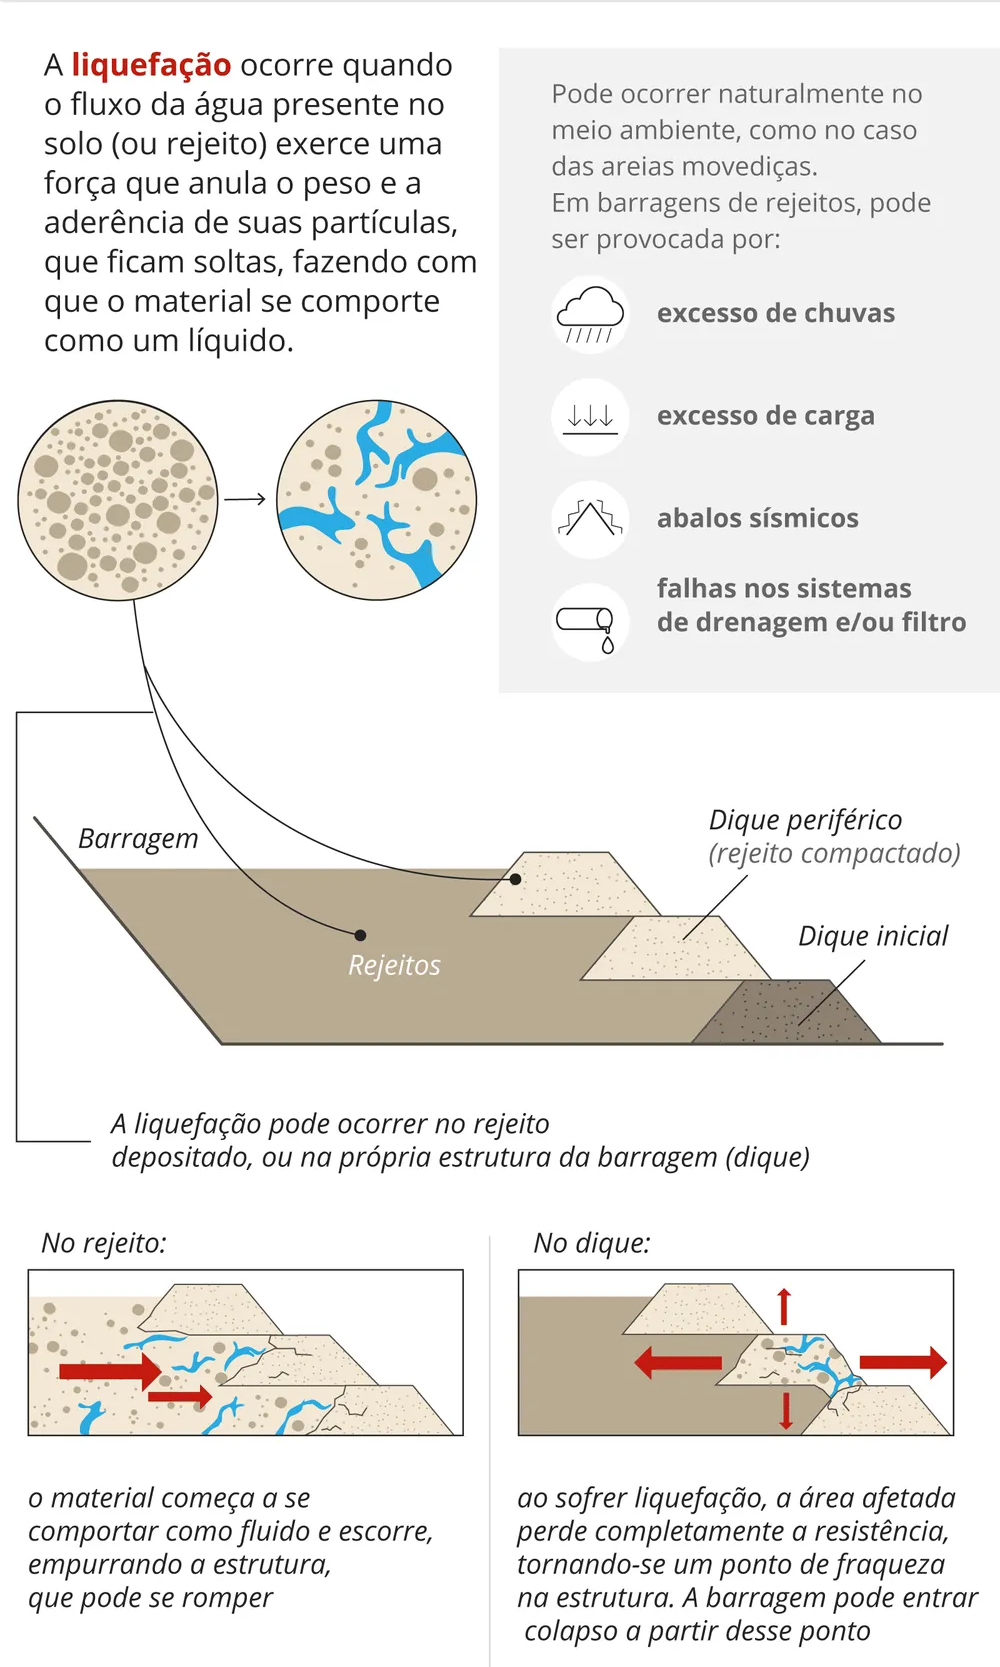
\includegraphics[width=0.5\textwidth]{figures/image_ruptura_liquefacao.png}}
    \caption{Ruptura de barragem por liquefação.}
    \label{fig:liquefacao}
    \fonte{\cite{freitas2019dissertacao}}
\end{figure}

O \textbf{galgamento} combina sobrepressões internas, causadas por drenagem inadequada, com erosão superficial por transbordamento. A ação simultânea das forças internas e externas gera um ciclo de retroalimentação que acelera a saturação interna e intensifica a erosão do paramento \cite{arnez1999avaliacao}, representada na Figura~\ref{fig:galgamento}.

\begin{figure}[H]
    \centering
    \fbox{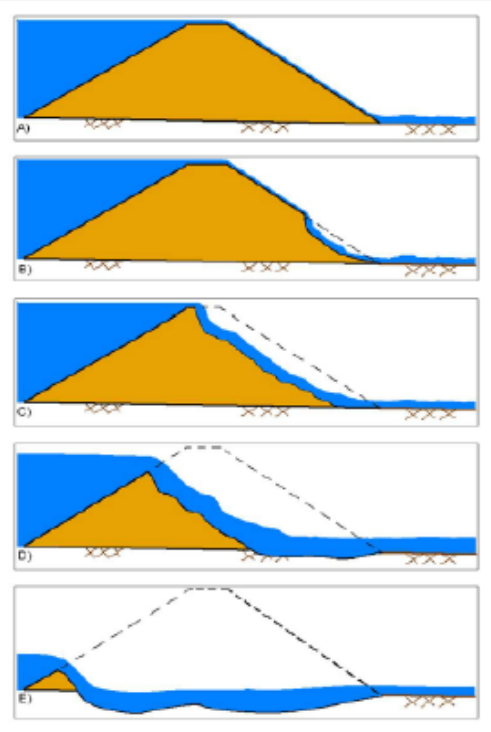
\includegraphics[width=0.4\textwidth]{figures/image_ruptura_galgamento.png}}
    \caption{Ruptura de barragem por galgamento.}
    \label{fig:galgamento}
    \fonte{\cite{lara2016metodologia}}
\end{figure}

A análise histórica de acidentes aponta a liquefação (46,7\%) e o erosão interna (\textit{piping}, 24,4\%) como principais causas técnicas de ruptura, sendo o gerenciamento inadequado o fator que permite o desenvolvimento dessas condições \cite{soares2010, duarte2008, carneiro2018}.

\subsection{Acidentes Internacionais de Referência}
\label{subsec:acidentes_internacionais}

O contexto internacional das falhas em barragens de rejeitos forneceu evidências fundamentais para a compreensão dos fatores de risco e a calibração de sistemas de monitoramento. \citeonline{rico2008mine} compilaram um banco de dados de 147 casos documentados de falhas em barragens de rejeitos em todo o mundo --- o levantamento mais abrangente disponível até aquela data --- identificando 15 causas distintas de ruptura e analisando sua distribuição geográfica e estatística.

Os resultados mostraram que causas meteorológicas, especialmente precipitação intensa, responderam por 25\% dos casos mundiais e chegaram a 35\% na Europa, configurando o fator de risco dominante no contexto europeu. A liquefação sísmica, segunda causa mundial com 14\% dos casos, mostrou-se praticamente ausente nas ocorrências europeias. O método construtivo a montante esteve associado a 76\% dos casos mundiais de ruptura --- dado que fundamentou as restrições regulatórias adotadas pelo Brasil após os desastres de 2015 e 2019 \cite{rico2008mine}.

Entre os casos documentados, o acidente de Merriespruit, ocorrido em Virginia, na África do Sul, em fevereiro de 1994, destacou-se como referência internacional para a compreensão do papel da precipitação pluviométrica na desestabilização de barragens de rejeitos. A estrutura, um dique de rejeitos auríferos construído pelo método a montante, estava em operação quando precipitação de aproximadamente 50\,mm em poucas horas elevou abruptamente o nível do lençol freático interno, reduzindo a resistência ao cisalhamento do material.

O colapso resultou no rompimento do dique, liberando cerca de 600.000\,m\textsuperscript{3} de rejeitos que percorreram as ruas do township vizinho e causaram a morte de 17 pessoas \cite{rico2008mine}. O caso de Merriespruit tornou-se amplamente citado na literatura técnica por evidenciar de forma inequívoca a relação entre eventos pluviométricos intensos e falhas de estruturas de contenção de rejeitos.

O limiar de 50\,mm/24h passou a ser adotado como referência crítica em modelos de avaliação de risco geotécnico, uma vez que eventos de precipitação dessa magnitude em curto intervalo de tempo representaram carga hidrológica capaz de comprometer a estabilidade de estruturas a montante mesmo sem a ocorrência de defeitos construtivos prévios \cite{rico2008mine}.

\subsection{Mariana}

Os rompimentos de barragens em Mariana (2015) e Brumadinho (2019) configuram os maiores acidentes ambientais e industriais da história do Brasil. Ambos envolveram estruturas sob gestão do grupo Vale e resultaram em perdas humanas, devastação ambiental e questionamentos profundos sobre os sistemas de licenciamento e fiscalização \cite{guitarrara2026rompimento}.

Em 5 de novembro de 2015, aproximadamente às 15h30min, rompeu-se a barragem do Fundão, no subdistrito de Bento Rodrigues, Mariana (MG). A estrutura pertencia à Samarco Mineração S/A, \textit{joint venture} de Vale e BHP Billiton Brasil, e o rompimento liberou rejeitos que alcançaram o Rio Doce \cite{brasil2024timeline}, apresentada nas Figuras~\ref{fig:rompimento_mariana} e ~\ref{fig:acidente_mariana}.

\begin{figure}[H]
    \centering
    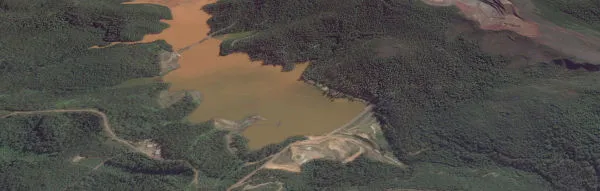
\includegraphics[width=0.8\textwidth]{figures/image35_rompimento_mariana.png}
    \caption{Imagem aproximada da barragem de Mariana antes do rompimento}
    \fonte{\citeonline{guitarrara2026rompimento_mariana}}
    \label{fig:rompimento_mariana}
\end{figure}

\begin{figure}[H]
    \centering
    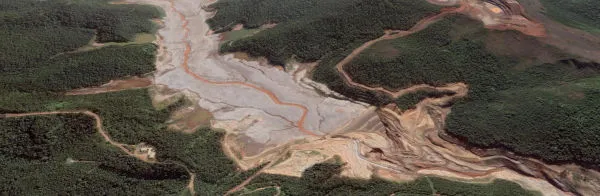
\includegraphics[width=0.8\textwidth]{figures/image37_acidente_mariana.png}
    \caption{Imagem aproximada da barragem de Mariana após o rompimento}
    \fonte{\citeonline{guitarrara2026rompimento_mariana}}
    \label{fig:acidente_mariana}
\end{figure}

A barragem havia sido construída de forma irregular a partir de 2007, sem apresentação adequada do projeto executivo à Fundação Estadual do Meio Ambiente (FEAM) de Minas Gerais, empregando o método de alteamento a montante sobre rejeitos pouco consolidados, o que comprometeu sua resistência estrutural \cite{estadominas2016irregular}. O acidente causou a morte de 19 pessoas e liberou entre 40 e 55 milhões de metros cúbicos de rejeitos, que contaminaram toda a bacia do Rio Doce --- cerca de 663~km, abrangendo 230 municípios nos estados de Minas Gerais e Espírito Santo --- e atingiram o Oceano Atlântico \cite{brasil2024timeline, projetomanuelzao2015}.

Os dados cadastrais da barragem do Fundão na FEAM estavam desatualizados desde 2012: o volume registrado correspondeu a apenas 2,65 milhões de metros cúbicos, cerca de 20 vezes inferior ao efetivamente liberado \cite{projetomanuelzao2015}.

Quanto às respostas institucionais, a criação da Fundação Renova pelas próprias mineradoras gerou controvérsia pela ausência de participação efetiva das vítimas; o acordo inicial foi anulado judicialmente em agosto de 2016 por iniciativa do Ministério Público Federal \cite{greenpeace2016valor}. As indenizações totalizaram cerca de R\$~8,71 bilhões até 2021 \cite{brasil2022indenizacoes} e, no plano criminal, o MPF denunciou 22 pessoas e as empresas envolvidas por crimes ambientais \cite{modelli2024brumadinho}.

Além disso, as consequências socioeconômicas para as comunidades atingidas incluíram destruição de propriedades, perda de meios de subsistência, agravamento de problemas de saúde mental e deslocamentos populacionais forçados \cite{estadominas2024alerta}.

\FloatBarrier
\subsection{Brumadinho}

Às 12h28min do dia 25 de janeiro de 2019, rompeu-se a Barragem I (B-I) da Mina Córrego do Feijão, controlada pela Vale S.A. em Brumadinho (MG), provocando em sequência o colapso das barragens B-IV e B-IV-A \cite{minasgerais2024historico}, representada nas Figuras~\ref{fig:momento_antes_brumadinho}, ~\ref{fig:momento_depois_brumadinho} e ~\ref{fig:acidente_brumadinho}.

\begin{figure}[H]
    \centering
    \includegraphics[width=0.8\textwidth]{figures/image33_momento_antes_brumadinho.png}
    \caption{Momento antes da tragédia em Brumadinho}
    \fonte{\citeonline{minasgerais2024historico}}
    \label{fig:momento_antes_brumadinho}
\end{figure}

\begin{figure}[H]
    \centering
    \includegraphics[width=0.8\textwidth]{figures/image34_momento_depois_brumadinho.png}
    \caption{Momento do rompimento da barragem na Mina Córrego do Feijão em Brumadinho}
    \fonte{\citeonline{minasgerais2024historico}}
    \label{fig:momento_depois_brumadinho}
\end{figure}

\begin{figure}[H]
    \centering
    \includegraphics[width=0.8\textwidth]{figures/image36_acidente_brumadinho.png}
    \caption{Acidente de Brumadinho}
    \fonte{\citeonline{warzynski2023barragem}}
    \label{fig:acidente_brumadinho}
\end{figure}

A estrutura havia sido construída em 1976 pela Ferteco Mineração, adquirida pela Vale em 2001 e ampliada em múltiplas etapas por diferentes projetistas, também pelo método a montante \cite{guitarrara2026rompimento}. Encontrava-se inativa desde 2015, classificada pela própria Vale como de ``baixo risco e alto potencial de danos'' \cite{guitarrara2026rompimento}.

O acidente causou 272 mortes oficiais, tornando-se o maior acidente de trabalho em perda de vidas no Brasil, e liberou aproximadamente 12,7 milhões de metros cúbicos de rejeitos, que atingiram o ribeirão Ferro-Carvão e o rio Paraopeba, comprometendo o abastecimento de água e a biodiversidade aquática da região \cite{guitarrara2026rompimento, minasgerais2024historico}.

A sirene de alerta jamais soou --- foi engolida pela onda de lama nos primeiros instantes do colapso devido à sua localização inadequada, sem plano de contingência eficaz. Laudos técnicos anteriores já recomendavam a instalação de radar de monitoramento de deslocamentos, tecnologia que poderia ter acionado o alarme a tempo \cite{taliberti2025tragedia, metropoles2019laudos}.

A resposta judicial, nesse caso, mostrou-se mais célere que em Mariana: as ações foram ajuizadas no mesmo dia do rompimento, com bloqueio imediato de recursos da Vale e imposição de obrigações emergenciais \cite{minasgerais2024historico}. A Vale firmou acordo de indenização de R\$~37,68 bilhões --- o maior da história do Brasil \cite{brasil2022indenizacoes}.

No entanto, a falta de punição efetiva aos responsáveis pela empresa e pela auditora Tüv Süd --- que emitiu laudos considerados fraudulentos --- permaneceu como ponto de crítica \cite{modelli2024brumadinho}.

\FloatBarrier
\paragraph*{Inovações Legislativas Pós-Brumadinho}

O contraste mais significativo entre as respostas institucionais está nas mudanças legislativas após Brumadinho. Minas Gerais aprovou a Política Estadual de Segurança de Barragens (PESB), determinando a descaracterização das estruturas a montante, ampliando a qualidade dos monitoramentos e tornando obrigatória a Declaração de Condição de Estabilidade (DCE) \cite{minasgerais2024historico}. A Lei n.º~14.066/2020 reformulou a PNSB em âmbito federal, proibindo formalmente o método a montante e fortalecendo os mecanismos de fiscalização \cite{brasil2020lei14066}.

% =============================================================
\section{Sistemas de alerta}
\label{sec:sistema_alerta}
% =============================================================

A taxa de falha das barragens de rejeitos é estimada em 1,2\% globalmente, valor significativamente superior aos 0,01\% das barragens convencionais de água \cite{stocks2019tailings}. Essa diferença impulsionou o desenvolvimento de sistemas de monitoramento mais sofisticados, que integram múltiplas tecnologias para detecção precoce de instabilidades.

\subsection{Sistemas de Monitoramento Atuais}

O monitoramento por sensoriamento remoto via satélite tem emergido como uma das tecnologias mais promissoras para alerta precoce. O projeto DAMSAT, desenvolvido pela UK Space Agency em parceria com a HR Wallingford, utiliza dados de satélite para monitorar deformações em barragens de água e rejeitos \cite{hrwallingford2021damsat}. Estudos demonstraram que a interferometria SAR (\textit{Synthetic Aperture Radar}) pode detectar acelerações de movimento que precedem colapsos, como evidenciado na análise retrospectiva de Brumadinho, onde tais movimentos foram identificados nos dois meses anteriores ao colapso \cite{naturecomm2020advanced}.

Os sistemas de monitoramento microsísmico proporcionam vigilância contínua 24/7 por redes de geofones. A Tetra Tech comissionou mais de 20 sistemas e instalou mais de 180 geofones em cerca de 50 estações sísmicas, principalmente em Minas Gerais, desde 2018 \cite{tetratech2023mitigating}. Pesquisas recentes mostram que mudanças de velocidade sísmica inferiores a 1\% se correlacionam com variações no nível d'água em lagoas de rejeitos adjacentes, abrindo caminho para alertas antecipados baseados em interferometria de ruído ambiente \cite{naturecomm2022monitoring}.

A tecnologia de sensoriamento distribuído por fibra óptica permite medições contínuas de temperatura, acústica e deformação ao longo de toda a extensão da estrutura por meio de um único cabo. Sistemas como o DamPulse (Silixa) e o SAAV Extend (Measurand) ilustram a aplicação dessas tecnologias em barragens de rejeitos \cite{silixa2024dampulse, rstinstruments2022tailings}.

A implementação desses sistemas em locais remotos demanda soluções de comunicação específicas. O sistema RAMJACK, por exemplo, utiliza comunicação em frequência sub-gigahertz para integrar piezômetros, extensômetros e inclinômetros wirelessly a um servidor central, reduzindo a necessidade de manutenção em campo \cite{ramjack2022tailings}.

O processamento dos dados massivos gerados por essas redes tem impulsionado a adoção de \textit{deep learning}. Li et al. desenvolveram um sistema com rede BiLSTM (\textit{Bidirectional Long Short-Term Memory}) para identificar padrões de instabilidade em séries temporais, obtendo RMSE de 0,09966 para entrada univariada, superior ao modelo MLP com RMSE de 0,10611 \cite{jing2022monitoring}. Plataformas de monitoramento integrado, como o sistema desenvolvido para a mina Zijinshan (China), unificam aquisição, transmissão, análise e alertas em uma única interface \cite{frontiers2022visualization}.

\subsection{Instrumentação Geotécnica Tradicional}

A instrumentação geotécnica tradicional continua sendo a base dos sistemas de monitoramento. Piezômetros medem a pressão neutra (poropressão) em diferentes profundidades e localizações da estrutura, enquanto inclinômetros detectam deslocamentos horizontais e verticais, identificando potenciais planos de ruptura \cite{geoscan2024sistema, ltec2024piezometros, ltec2025inclinometros}.

Esses instrumentos apresentam, contudo, uma limitação crítica: a dependência de leituras manuais periódicas, que compromete a continuidade e a atualidade dos dados. Essa inadequação foi evidenciada nos acidentes de Mariana e Brumadinho, e impulsionou o desenvolvimento de soluções automatizadas \cite{anm2019relatorio, ibram2020tecnologias}.

Em Mariana, o sistema da barragem do Fundão era genérico e baseado apenas em piezômetros para determinação de níveis d'água, sem instrumentação adequada e sem simulações específicas de evacuação \cite{sequencia2024sismografico, geoscan2024sistema}. 

Em Brumadinho, a sirene de alerta foi engolida pela onda de lama nos primeiros segundos do colapso por estar posicionada inadequadamente, sem plano de contingência eficaz. Laudos técnicos já recomendavam a instalação de radar de monitoramento de deslocamentos, tecnologia que poderia ter acionado o alarme a tempo \cite{taliberti2025tragedia, metropoles2019laudos}.

\subsection{Estudo de Caso Internacional: Enchentes no Texas (2025)}

Na madrugada do dia 4 de julho de 2025, feriado da Independência dos Estados
Unidos, enchentes repentinas devastaram a região central do Texas, epicentrada
no Condado de Kerr e no vale do Rio Guadalupe. O evento causou mais de 100
mortes, incluindo pelo menos 27 meninas e monitoras do acampamento cristão
Camp Mystic, e expôs de forma inequívoca as consequências da ausência de um
sistema integrado de alerta precoce em uma área historicamente reconhecida
como de alto risco \cite{cnnbrasil2025texas, bbc2025texas, horadopovo2025texas}.

O contexto geográfico da região amplifica qualquer evento pluviométrico
extremo. A área, conhecida como \textit{Flash Flood Alley} (``Beco das Enchentes
Relâmpago''), caracteriza-se por colinas íngremes, solo semiárido com baixa
capacidade de absorção e cursos d'água rasos que enchem rapidamente. Quando
riachos em cheio convergem para o Rio Guadalupe, formam massas d'água
capazes de arrastar casas, veículos e pessoas \cite{bbc2025texas}. Na madrugada
da tragédia, o Rio Guadalupe subiu aproximadamente 9 metros em menos de
uma hora, e a área de Hunt recebeu cerca de 165 milímetros de chuva em apenas
três horas --- volume equivalente ao esperado para todo um verão na região
\cite{cnnbrasil2025texas}.

O Serviço Nacional de Meteorologia dos Estados Unidos (NWS) emitiu alertas
de inundação para o Condado de Kerr desde a tarde da quinta-feira, dia 3, e
às 01h14 do dia 4 publicou aviso de enchente repentina com ``risco de vida''
para 30.000 pessoas. Apesar disso, as autoridades locais só iniciaram a
divulgação de alertas nas redes sociais após as 05h00, e a cidade de Kerrville
recebeu alerta de emergência apenas às 05h34 --- horas depois de o rio já
estar em colapso. Boa parte da população foi pega dormindo, sem sirenes,
sem rádio de emergência e sem sinal de celular suficiente para receber os
avisos enviados por SMS \cite{globo2025texas, horadopovo2025texas,
cnnbrasil2025texas}.

A raiz estrutural do desastre, contudo, não foi o evento climático em si, mas
uma decisão administrativa tomada ao longo de mais de uma década. O
Condado de Kerr recusou sistematicamente a implantação de um sistema
moderno de alerta contra inundações. Em 2017, uma proposta orçamentária
de US\$~1 milhão para instalação de sensores de nível d'água, sirenes e
comunicação integrada foi rejeitada com o argumento de custo excessivo ---
em um condado com orçamento anual de US\$~67 milhões. 

O tema voltou à pauta em maio de 2025, mas sem decisão concreta \cite{metsul2025texas}.
A professora Avantika Gori, da Universidade Rice, que lidera projeto federal
de resiliência a enchentes em áreas rurais do Texas, foi direta ao avaliar a
situação: ``Se o condado tivesse um sistema de alerta em funcionamento,
estaria muito mais preparado. Estamos praticamente cegos quando se trata
de identificar áreas vulneráveis'' \cite{metsul2025texas}. O próprio Diretor de
Emergências do Condado, Rob Kelly, admitiu publicamente: ``Não temos um
sistema de alerta precoce. Ninguém sabia que uma enchente dessas
aconteceria'' \cite{horadopovo2025texas}.

O contraste com o município vizinho de Wimberley é revelador: após uma
enchente em 2015 que matou 10 jovens em um acampamento religioso,
Wimberley adotou um sistema integrado de sensores e comunicação com apoio
de agências federais. O condado de Kerr, que tinha o mesmo histórico de risco,
não seguiu o mesmo caminho. Durante as enchentes de 2025, a cidade de
Comfort --- localizada mais abaixo no mesmo Rio Guadalupe e equipada com
sirenes --- não registrou mortes, atribuindo parcialmente esse resultado ao
acionamento tempestivo dos alarmes \cite{metsul2025texas}.

Agravando o quadro, investigações posteriores revelaram que cargos de
hidrólogos e meteorologistas nos escritórios do NWS no Texas haviam sido
reduzidos por cortes promovidos pelo governo federal a partir de janeiro de
2025. A ausência desses profissionais dificultou a coordenação com as
autoridades locais nas horas críticas que antecederam o pico da enchente
\cite{bbc2025texas, globo2025texas}.

O caso do Texas é um exemplo internacional recente e documentado de como
a omissão em investir em sistemas de monitoramento e alerta precoce --- mesmo
em regiões com histórico comprovado de risco --- pode amplificar
catastroficamente os impactos de eventos hidrológicos extremos. A lição
converge diretamente com as deficiências identificadas em Mariana e
Brumadinho: em todos os casos, a tecnologia de alerta existia, o risco era
conhecido, e a decisão de não implementar ou manter os sistemas precedeu
a tragédia.

\subsection{Sistemas Automatizados de Monitoramento}

A implementação de sistemas automatizados tem reduzido a dependência de inspeções manuais. O Cleveland Dam (North Vancouver, Canadá), classificado como de consequência extrema, utiliza rede complexa de piezômetros, inclinômetros, sensores de turbidez e fluxo integrados via SCADA \cite{klohn2021surveillance}. 

A Worldsensing desenvolveu o sistema LSG6, que simplifica o monitoramento de barragens de rejeitos ao integrar instrumentos geotécnicos com comunicação \textit{wireless} de longo alcance, reduzindo significativamente o custo e a necessidade de envio de técnicos ao campo \cite{worldsensing2024canadian, minedesign2021tailings}.

\subsection{Desafios Regulatórios Internacionais}

A ausência de regulamentação internacional uniforme para barragens de rejeitos representa um desafio para a padronização dos sistemas de alerta. Não existe órgão internacional independente regulamentando barragens de rejeitos, resultando em abordagens fragmentadas \cite{londonmining2021explainer, earthworks2024safety}. 

Os desastres brasileiros expuseram essas limitações e motivaram a criação do \textit{Global Industry Standard on Tailings Management}, desenvolvido conjuntamente pelo ICMM, PNUMA e PRI \cite{icmm2020global}. Países como Canadá, Austrália e Chile desenvolveram protocolos abrangentes com monitoramento automatizado, sistemas de comunicação redundantes e planos de evacuação estruturados \cite{bentley2025solucoes}.

\subsection{Perspectivas Futuras}

A evolução dos sistemas de alerta aponta para a integração de múltiplas tecnologias de sensoriamento com análise de dados avançada. A aplicação de gêmeos digitais permite criar modelos virtuais que incorporam dados de diferentes fontes e realizam simulações preditivas em tempo real. 

A integração de sensores terrestres com monitoramento por satélite está criando capacidades multi-escala, enquanto algoritmos de aprendizado de máquina prometem identificar precursores de falha não detectáveis por análises convencionais \cite{internationalwater2024digital, sequencia2024tempo}. 

Protocolos de comunicação baseados em IoT e sistemas de resposta automatizada devem reduzir o tempo entre a detecção de anomalias e a implementação de medidas corretivas, ampliando a segurança das comunidades que vivem no entorno de barragens de rejeitos \cite{ufpr2021simepar, radaz2024revolucionando}.

Nessa direção, a última década tem sido marcada pela integração de tecnologias digitais nos sistemas de governança ambiental da mineração. A Resolução ANM n.º~95/2022 tornou obrigatória a revisão periódica de segurança e o monitoramento em tempo real de barragens, incorporando recomendações internacionais do ICOLD e padrões canadenses de gestão de rejeitos \cite{anm2022resolucao95, icold2022tailings, mac2021guide}. 

Tecnologias como sensoriamento remoto por satélite, drones e inteligência artificial para análise preditiva de riscos têm sido progressivamente integradas ao marco regulatório brasileiro e internacional \cite{darzi2024transformacao}.